\section{Implementation and Results}
The framework of our system is implemented with Python with Scikit-learn library for dimension reduction and clustering.
As we are currently working with data with reduced size, the data are locally stored in the hard disk of an local workstation.
All the computation are undertaken by one core of a Intel Core i5 3.2 Ghz quad processor.
As we are aiming at identify and visualize similar climate patterns for the current milestone, we do not have any annotated groundtruth from the dataset.
In order to achieve sanity check for our algorithms and prepare for the comming large-scale experiment, we use an ambiguious but effective measure.
More specifically, we verify the result with our prior geology knowledge. E.g. we verify whether different clusters are constructed along China's coastal and inland areas.
In the following subsection, we will first analyse clustering and visualization results for different continents.
Extended discussion about features and parameters in clustering and dimension reduction algorithms will follow with concrete examples.

\subsection{Clustering Result Verification}
\begin{figure}
    \centering
    \begin{tabular}{c c}
        \includegraphics[width=.45\linewidth]{./figure/Ave_60_comp_75_clu_USA.png}
        & 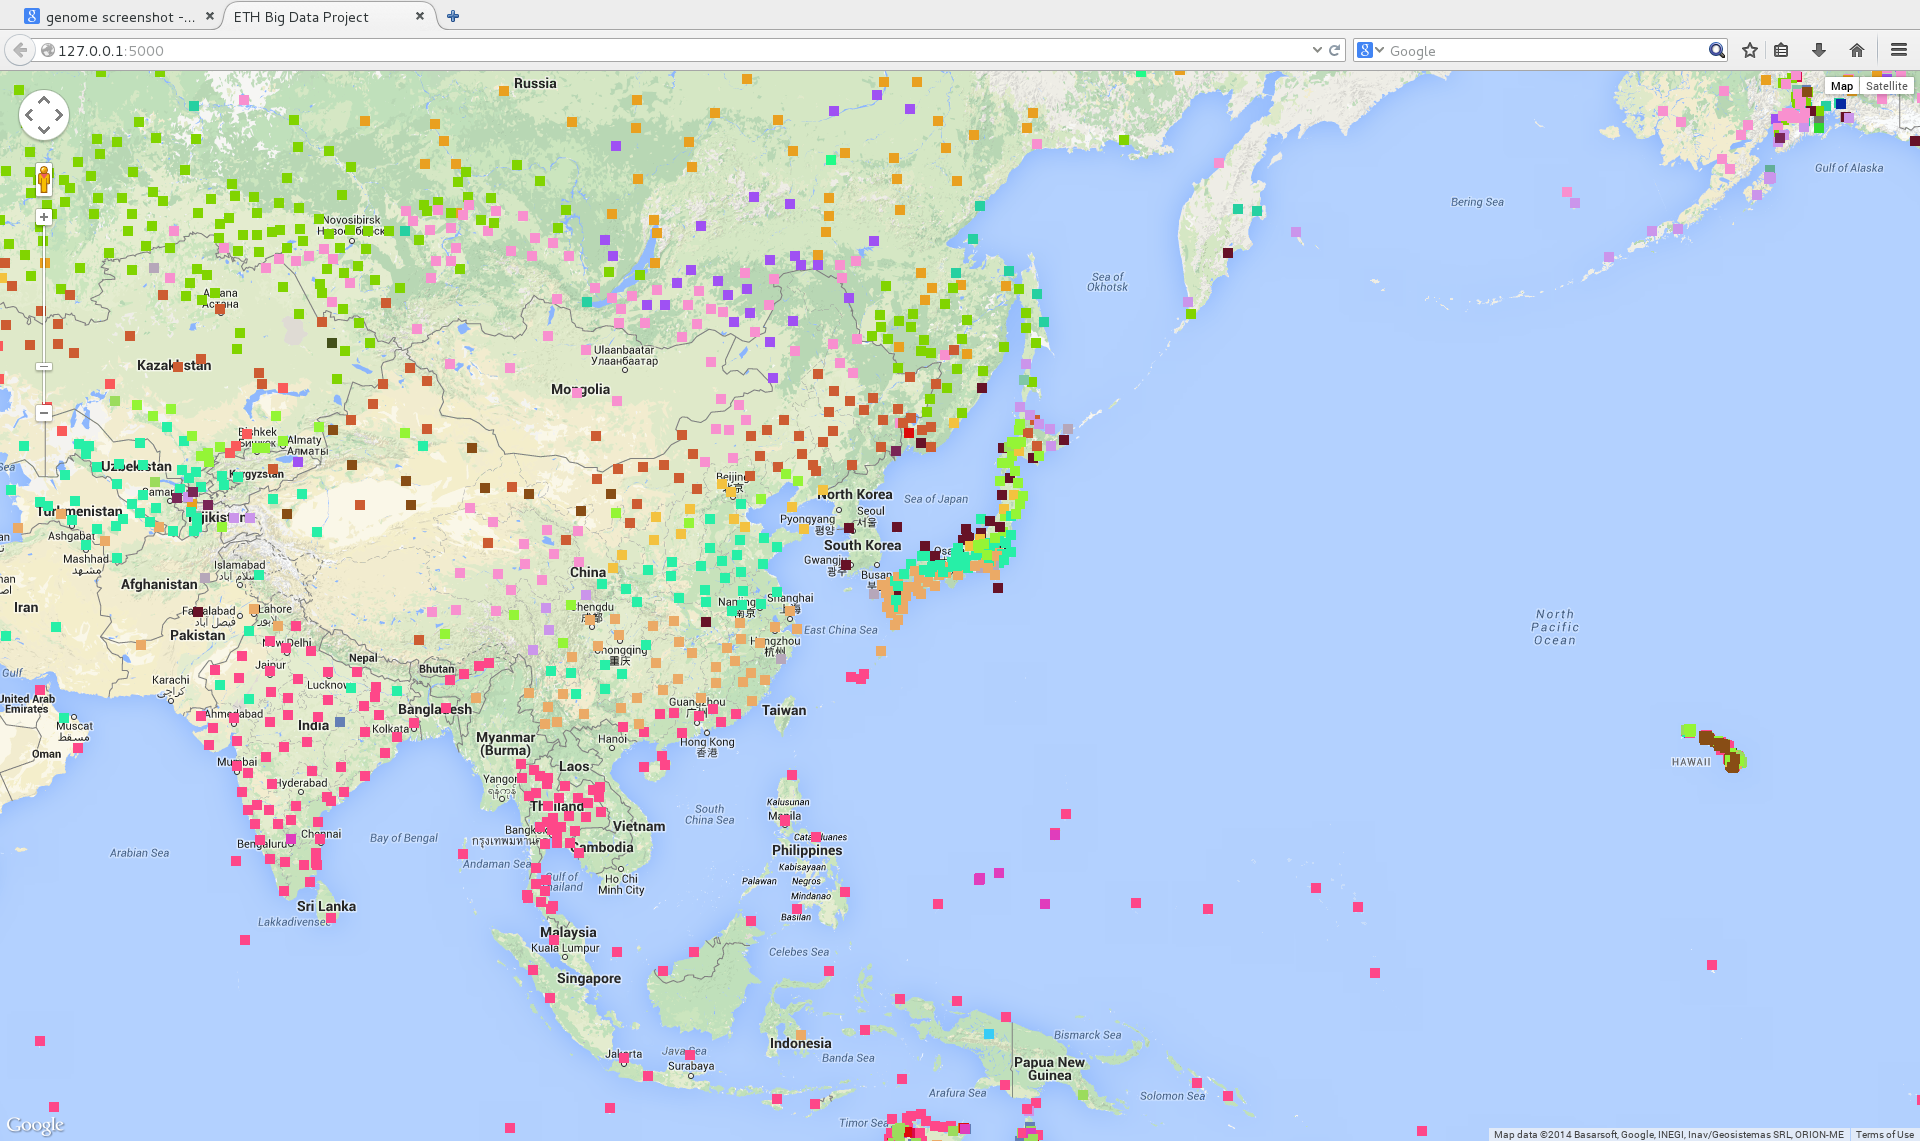
\includegraphics[width=.45\linewidth]{./figure/Ave_60_comp_50_clu_Asia.png}
    \end{tabular}
    \caption{Left: Climate pattern clustering for North American Continent with 75 clusters. Right: Climate pattern clustering for Asia with 50 clusters.}
    \label{fig:AsiaUSAVer}
\end{figure}

When verifying the results with our prior geology knowledge, we use 60 dimensional mean-value-based feature with 75 cluster components for North American continent and with 50 cluster components for Asia. We use different cluster numbers to better illustrate the results as the intrinsic climate patterns are different on the two continents.

As the climate pattern of North America shown in Fig. \ref{fig:AsiaUSAVer}, we can observe an obvious division of Areas closer to the Pacific Ocean and Atlantic Ocean. It is possibly a direct consequence of the different monsoon pattern which are closely related to the two oceans. With closer observation, we can identify three finer-grain clusters. Around Florida, a cluster is formed for the perfect climate pattern of costal vacations. Around the Great Lakes, on the contrary, we observe an patterns which corresponds to extremely code weather in winters. In addition, the light pink region near Nevada surrounded by deep pink patterns reveals the existence of dry climate in desert areas.

In the visualization of Asia climate patterns, we can observe a large cluster of tropical and subtropical climates on South Asia subcontinent and Southeast Asia. Other climate clusters, which distribute in alignment with different latitude range, can be analogously identified. Interestingly, we can observe a three-step structure starting from Chinese coast towards inland of Asia-Europe Continent. The steps corresponds to costal areas, inland plains and inland plateaus, which well explained the variation of height above sea level.

\subsection{Variance-based Features}
\begin{figure}
    \centering
    \begin{tabular}{c c}
        \includegraphics[width=.45\linewidth]{./figure/Ave_60_comp_75_clu_USA.png}
        & 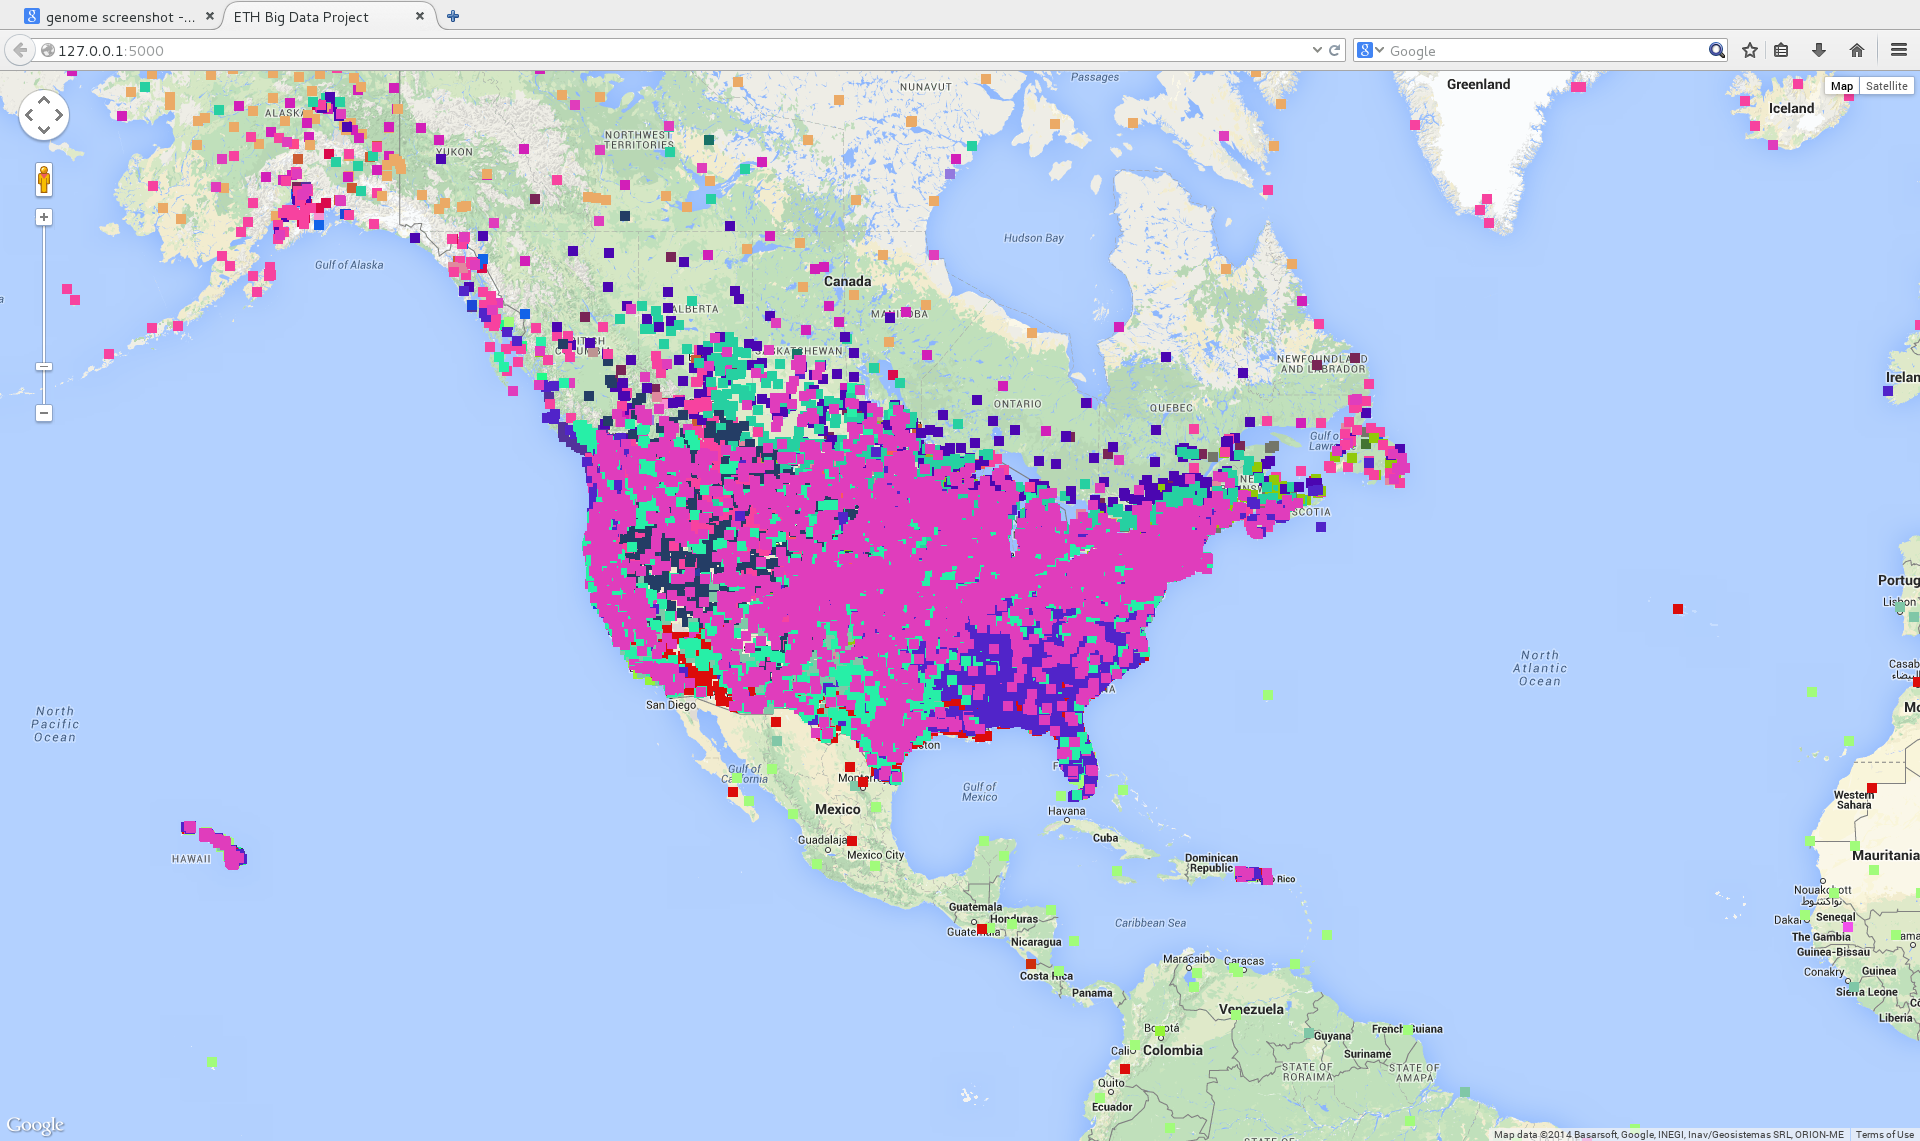
\includegraphics[width=.45\linewidth]{./figure/Var_120_comp_75_clu_USA.png}
    \end{tabular}
    \caption{Clustering pattern with 75 cluster for North America. Left: 60 dimensional mean-value based features. Right: 120 dimensional mean-value and variance based feature.}
    \label{fig:VarFeature}
\end{figure}
In addition to our mean-value-based feature, we also conduct experiments with additional variance-based Features. In Fig. \ref{fig:VarFeature}, we illustrate different result with and without variance-based features. When variance-based features are included, the finer-grain clusters near Florida, around Nevada and around the Great Lakes diminish. The difference between eastern and western parts is also eliminated. These facts are indicators of the weaker discriminability than mean-value based features. Intuitively, mean-value based features represents the average climate characteristics of different measure stations. However, one stations in the tropical region and the other in the Arctic may both have very stable measurements in each month, which results in similar small values for variance-based features. Thus the additional variance-based features contributes more noise than information which eventually degrade the quality of clustering.

\subsection{Number of Clusters}
\begin{figure}
    \centering
    \begin{tabular}{c c}
        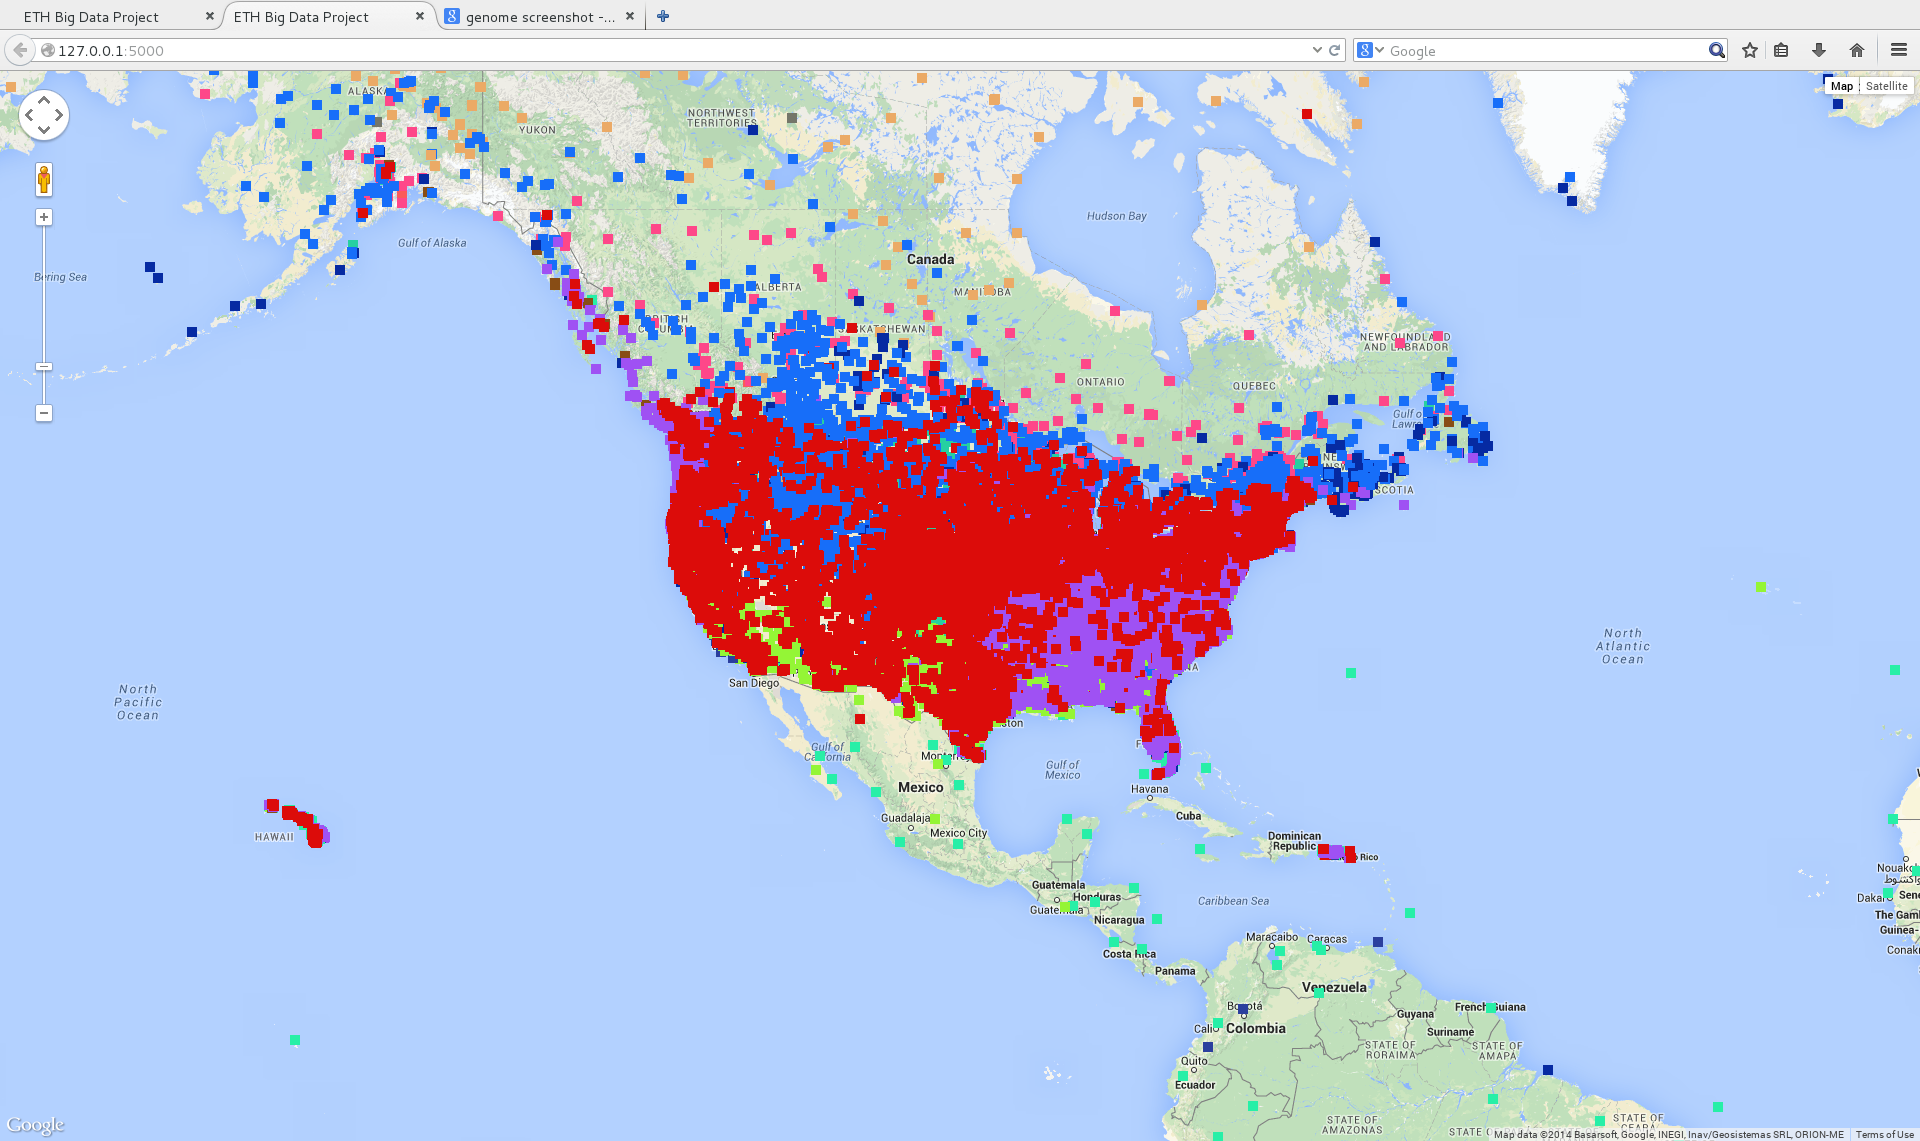
\includegraphics[width=.45\linewidth]{./figure/Ave_60_comp_15_clu_USA.png}
        & \includegraphics[width=.45\linewidth]{./figure/Ave_60_comp_75_clu_USA.png}
    \end{tabular}
    \caption{Clustering pattern with 60 dimensional mean-value-based feature for North America. Left: clustering with 15 components. Right: clustering with 75 components.}
    \label{fig:CluNum}
\end{figure}

Different continents have different geology characteristics in many properties, which results in different intrinsic cluster structures of climate patterns. Selecting a well-approximated number of clusters is essential to effectively mine climate patterns in a specific region. E.g. in Fig. \ref{fig:CluNum}, we can find fine-grain structures in Forida, around Nevada with 75 clusters while lose these details with only 15 clusters.

\subsection{Feature Dimension Reduction}
\begin{figure}
    \centering
    \begin{tabular}{c c}
        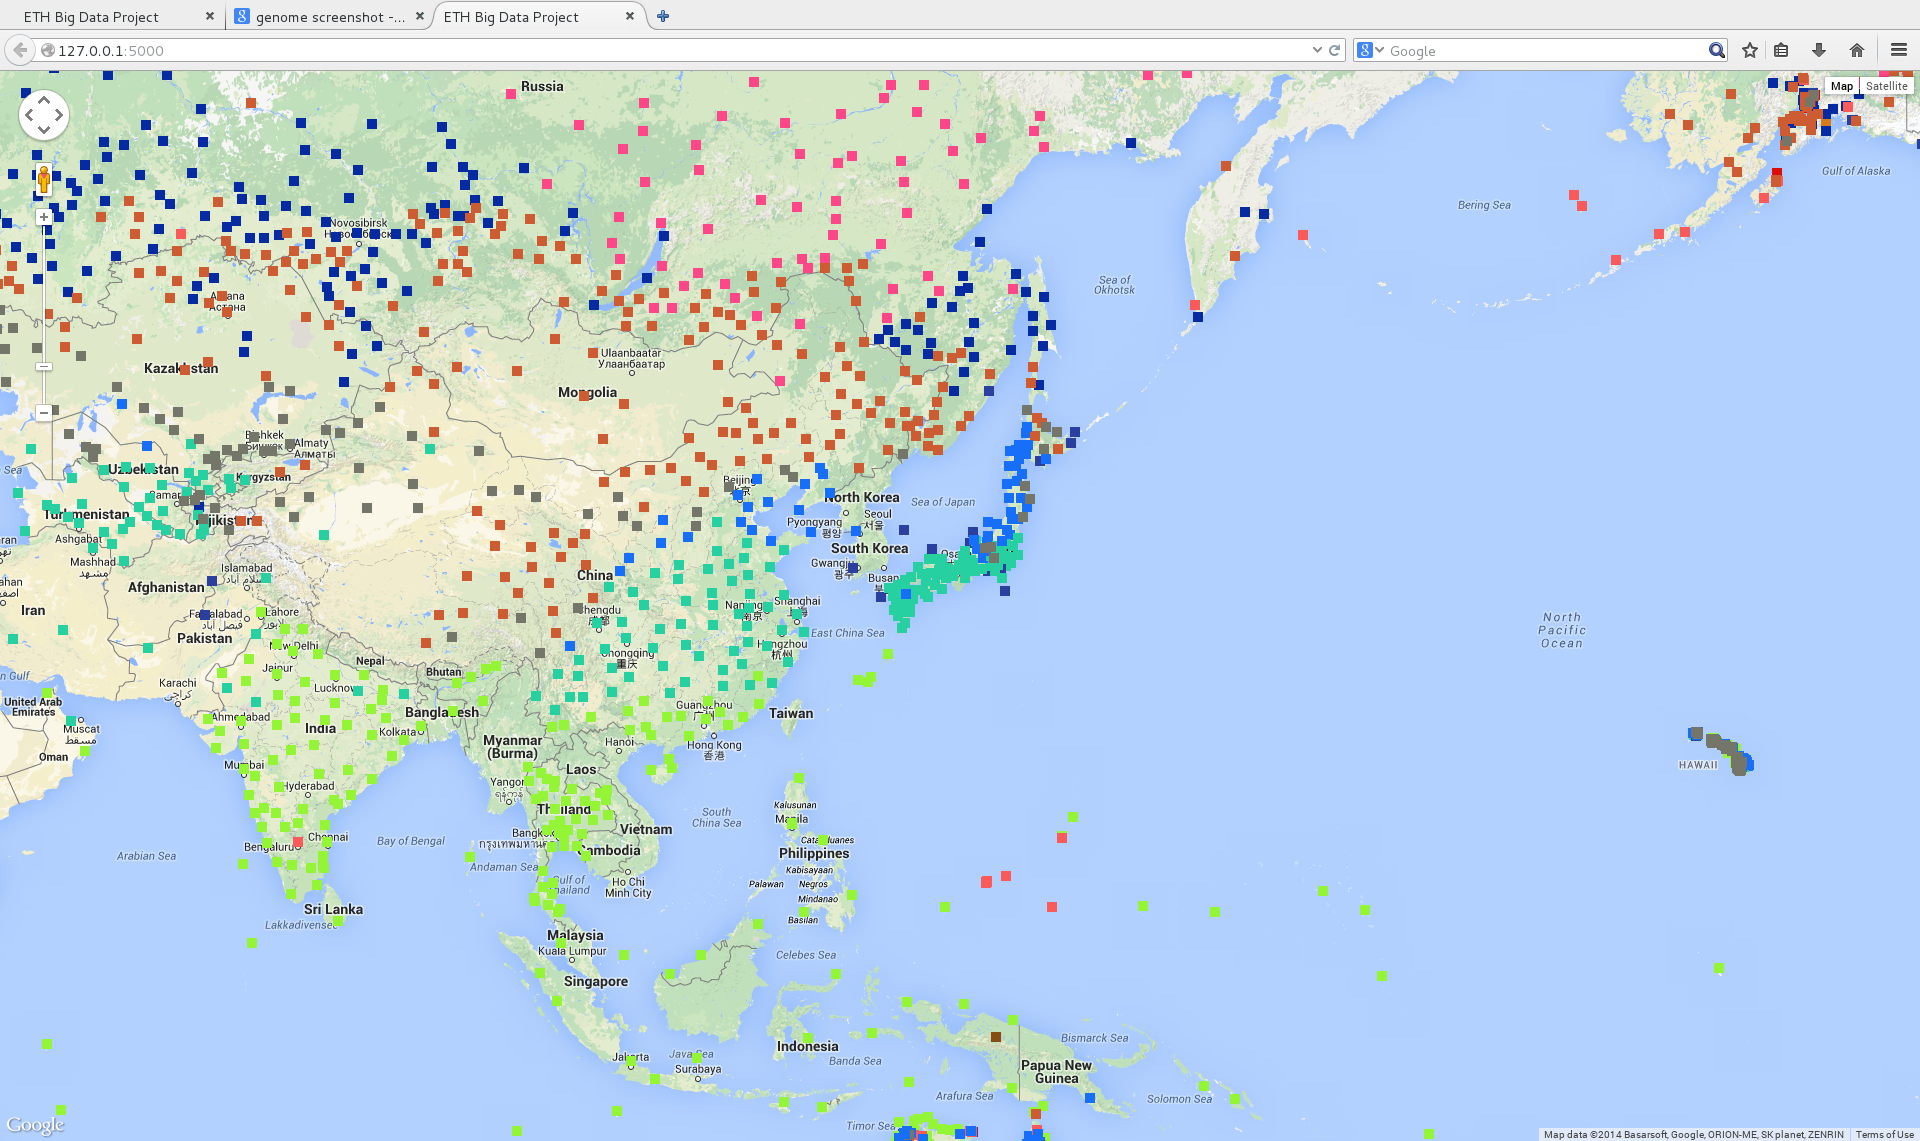
\includegraphics[width=.45\linewidth]{./figure/Ave_25_comp_15_clu_Asia.png}
        & 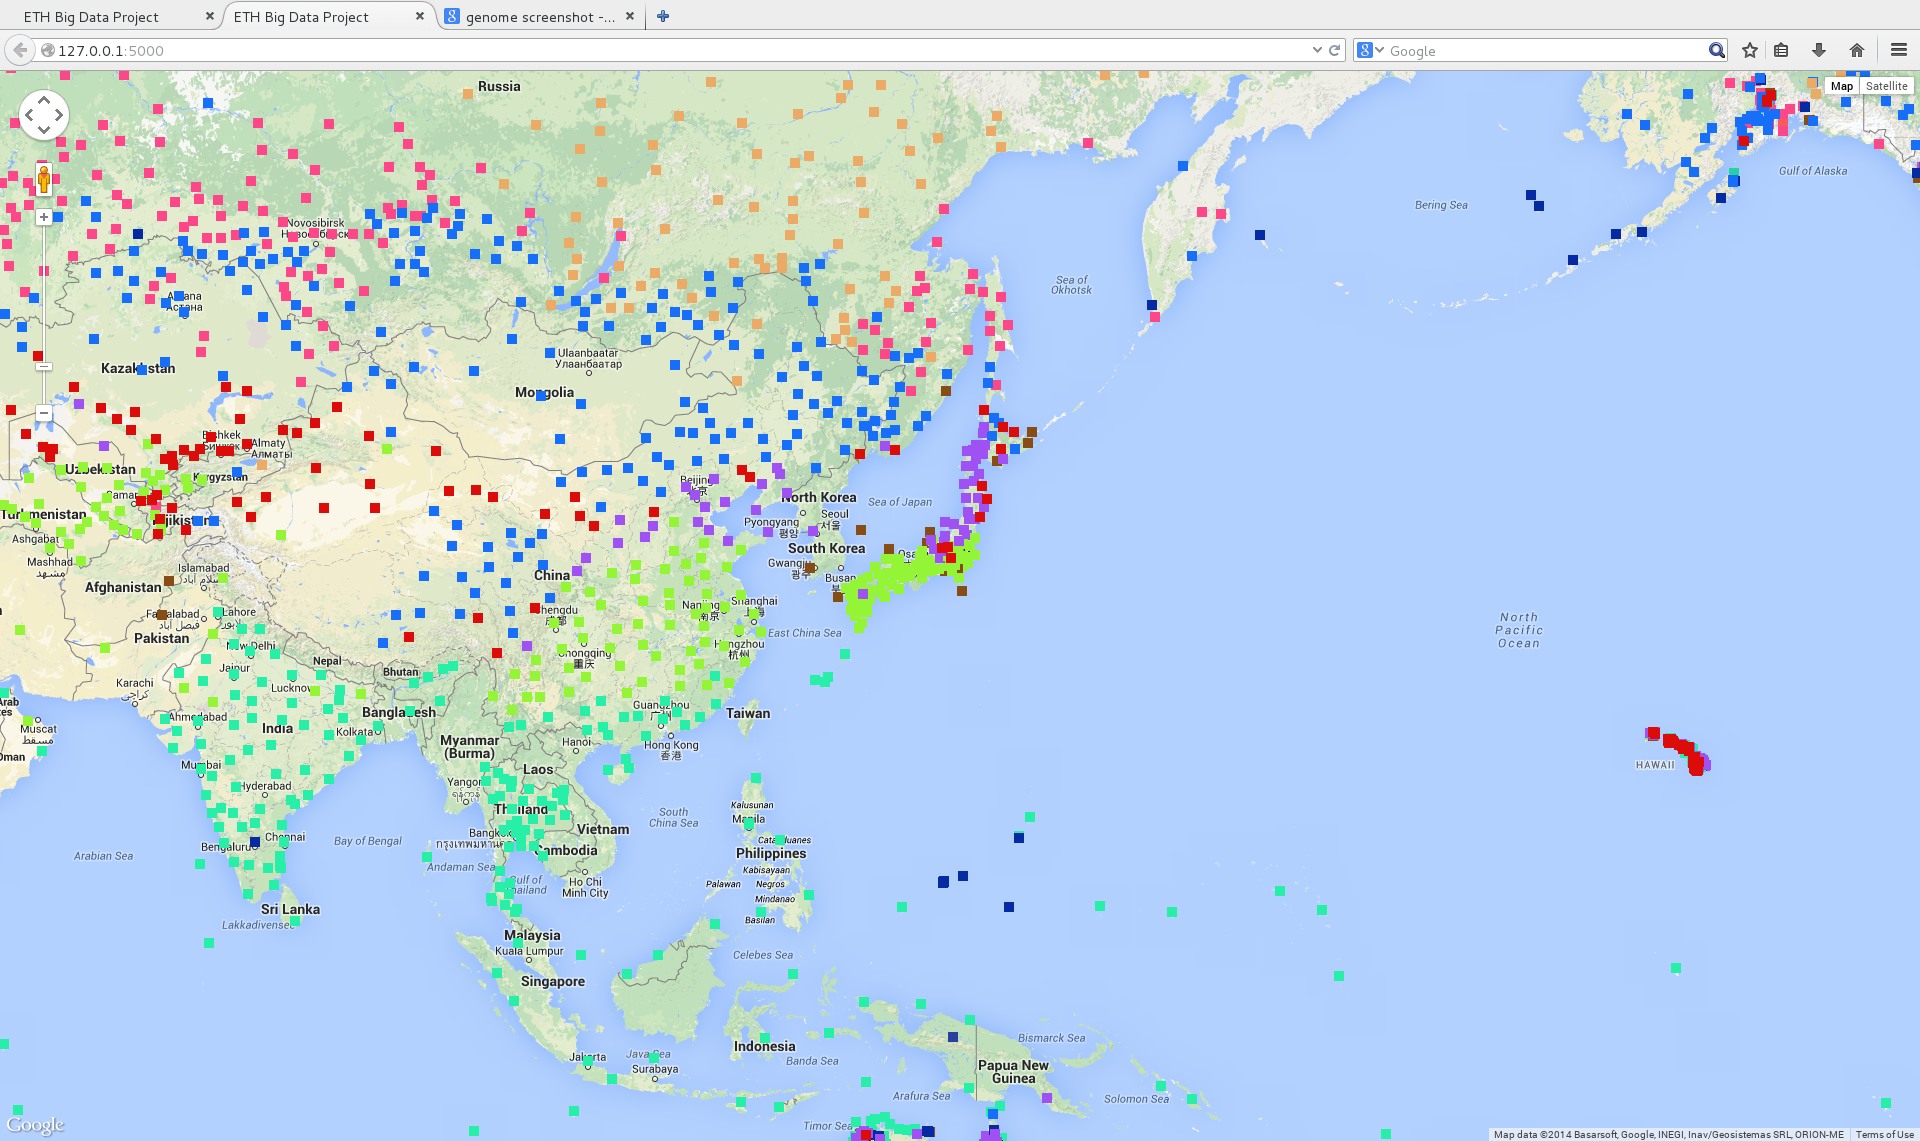
\includegraphics[width=.45\linewidth]{./figure/Ave_60_comp_15_clu_Asia.png}
    \end{tabular}
    \caption{Clustering pattern with 15 cluster for North America. Left: 60 dimensional original mean-value based features. Right: 25 dimensional feature reduced by PCA from mean-value-based feature.}
    \label{fig:VarFeature}
\end{figure}
In the next milestone, we will have to leverage data spanning over 90 years instead of over one year, reducing the computing overhead is essential for efficient analysing. Our major computation is exerted by clustering. Thus effectively reduce feature dimension is not only a way to eliminate noise but also a key step towards tractable computing. In our experiment, we test the effect of PCA on the model with 15 clusters. In Fig. \ref{fig:VarFeature}, by checking clusters in China, in Japan and in Northern Asia, we can find 25 dimensional features, reduced from original 60 dimensional mean-value-based features, produce similar results with similar quality while reducing more than half of the computing time of clustering. 




